\documentclass[journal]{IEEEtran}

% helps to remove under full and over full hboxes
\usepackage[activate={true,nocompatibility},final,tracking=true,kerning=true,spacing=true,factor=1100,stretch=10,shrink=10]{microtype}

% make it fit on two pages
\linespread{0.97}

\usepackage{amsmath}
\usepackage{bm}
\usepackage{amssymb}
\usepackage{algorithm}
\usepackage{algorithmic}
\usepackage{stfloats}

\ifCLASSINFOpdf
   \usepackage[pdftex]{graphicx}
\else
   \usepackage[dvips]{graphicx}
\fi

\ifCLASSOPTIONcompsoc
  \usepackage[caption=false,font=normalsize,labelfont=sf,textfont=sf]{subfig}
\else
  \usepackage[caption=false,font=footnotesize]{subfig}
\fi

\usepackage[style=ieee,maxbibnames=1,minbibnames=1,maxcitenames=1,mincitenames=1,backend=biber,defernumbers=false]{biblatex}
\addbibresource{my_TOF_model.bib}

\begin{document}
\title{Impact of Axial Ring Splitting on Image Quality for the Cost Reduction of Total-Body PET}
\author{N.~Efthimiou~(\IEEEmembership{Member~IEEE}),
        A.C.~Whitehead~(\IEEEmembership{Student~Member~IEEE}),
        M.~Stockhoff~(\IEEEmembership{Student~Member~IEEE}), 
        C.~Thyssen~(\IEEEmembership{Student~Member~IEEE}),
        S.J.~Archibald
        and~S.~Vandenberghe~(\IEEEmembership{Senior~Member~IEEE})%
        
        \thanks{This project was supported in part by the European Cooperation for Science and Technology Action TD1401: Fast Advanced Scintillation Timing}%
        \thanks{This project was supported in part by the Daisy Appeal Charity.}%
        \thanks{N.~Efthimiou and S.J.~Archibald are with the PET research centre, Faculty of Health Sciences, University of Hull, Hull, HU6~7RX, UK (contact: \texttt{n.efthymiou@hull.ac.uk}).}%
        \thanks{A.C.~Whitehead is with the Institute of Nuclear Medicine, University College London, London, NW1~2BU, UK}%
        \thanks{M.~Stockhoff, C.~Thyssen  and S.~Vandenberghe are with Ghent University, Ghent, Belgium.}%
        \thanks{We thank Dr. A. Allam and his family for the generous donation to help found the PET Research Centre at the University of Hull and for their continued support.}}%

\maketitle
\vspace{-1cm}
    
\IEEEpeerreviewmaketitle
\begin{abstract}
Total-Body PET (TB-PET), due to high sensitivity, provides the means for simultaneous imaging of distant organs, fast kinetics, use of short-lived isotopes and paediatric applications. Recently the first TB-PET scanner was presented and the first results were impressive. However, the cost of a TB-PET scanner is prohibiting for many clinics and research institutions. Therefore we propose a flexible detector configuration which will increase the axial field of view and keep the total cost low. Axial ring splitting separates the full rings into rings with only the even numbered detectors and the odd. In this investigation three configurations were considered (a) half length full rings (b) double length - split rings (c) double length - full rings. It was shown that configuration C demonstrated the highest prompt count rate, as expected. Configuration A was marginally better than configuration C. The same trends were observed in terms of noise equivalent count rate. Images reconstructed with OSEM demonstrated the improved image quality and noise properties of the long scanner configuration over classic PET. 
\end{abstract}
    
\begin{IEEEkeywords}
    Total-Body~PET, Monte~Carlo, Image~reconstruction, Noise~Equivalent~Count~Rate
\end{IEEEkeywords}

\section{Introduction}
Total-Body PET (TB-PET) scanners are long axial Field-of-View (FOV) scanners, designed with the aim of imaging large portions of the body without bed movement\cite{Moskal2016PotentialSystem, Cherry2018Total-BodyCare.}. The scientific interest in the novel imaging possibilities and technological challenges, has been surging. Finally, last year, the first commercial TB-PET scanner for human scanning was presented and the first scans reported\cite{Leung2018PerformanceScanner, Badawi2019FirstScanner.}.

TB-PET scanners allow simultaneous imaging of distant organs, adding the possibility of investigating their mutual interactions. Other key areas include fast kinetics, injection of high activities of short-lived isotopes and the possibility of paediatric applications.

The aim of this work is to try to find a more cost effective way to build a TB-PET scanner.
In particular we investigated the possibility of a chess-like arrangement of detectors, by splitting each ring into a ring with the even detectors and a ring with the odd detectors (Fig.~\ref{fig:configs}). Hence, this will double the axial FOV while the number of detectors remains the same. 

\section{Materials and Methods}
The GATE~\cite{Jan2004} Monte Carlo toolkit was used for the simulation process. STIR~\cite{Thielemans2012P} was used for reconstruction and the processing of sinograms.

Three configurations were considered. A long axial FOV scanner with an axial length of $626$mm, a split ring configuration, where interchangeably rings lack either the odd or the even detectors, with an axial length of $1252$mm and finally a standard TB-PET scanner with full rings axial length $1252$mm. The configurations were named: \texttt{Config.A}, \texttt{Config.B} and \texttt{Config.C}, respectively. The three configurations are illustrated in Fig~\ref{fig:configs}. 

Briefly, the system model is composed of blocks of $8 \times 8$ LYSO crystals with size $4 \times 4 \times 20$mm$^3$.  Each module either had one block (\texttt{Config.A}), a combination of block and gap (\texttt{Config.B}) or two blocks (\texttt{Config.B}).

The digitiser was taken from a validated Philips Vereos model~\cite{Rausch2019PerformanceStandard} due to its high resoluation timing properties. 

Because the NEMA NU-2012~\cite{NationalElectricalManufacturersAssociation2012Performance2-2012} protocol is not optimised for such long scanners adaptations were made to the protocol. In particular the count losses phantom, which in NEMA has a length of $700$mm, was extended to $1500$mm, in order to provide a fair comparison between the long scanners and highlight the benefits of the longer axial FOV. In addition, the XCAT digital anthropomorphic phantom~\cite{Segars20104DResearch} was also simulated.

\begin{figure}
    \centering
    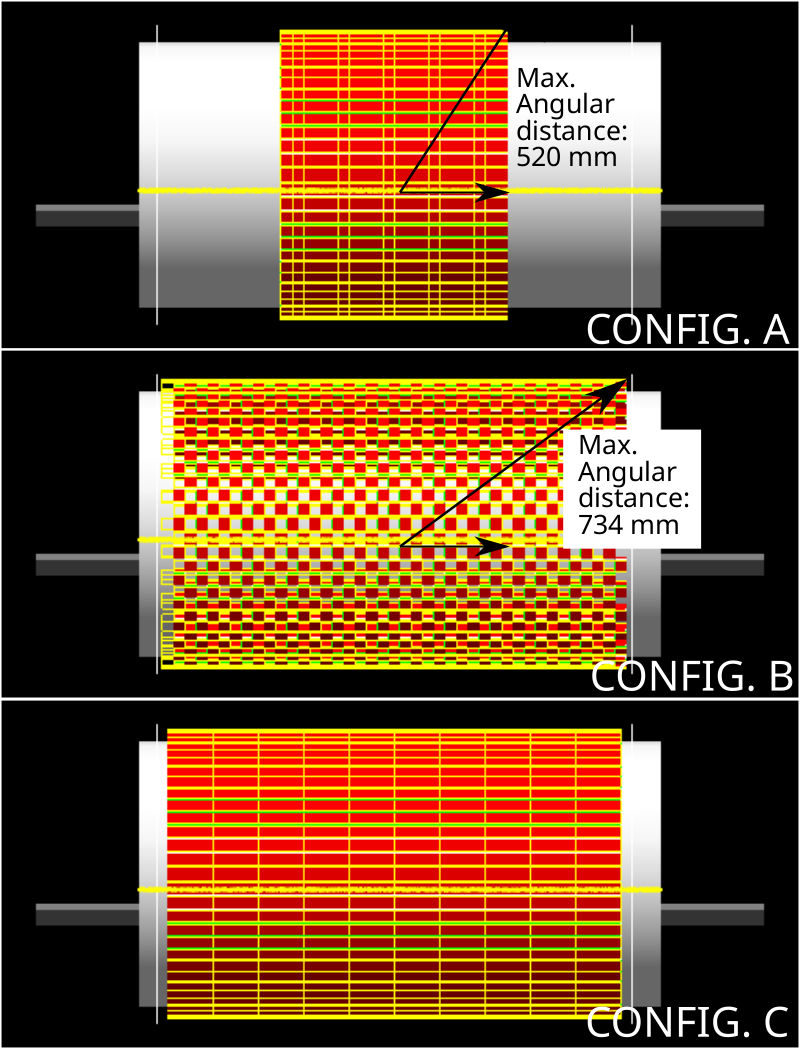
\includegraphics[width=0.9\linewidth]{dfd.png}
    \caption{The three configurations considered in this investigation. \textit{(The white cylinder is used for visualisation purposes)}}
    \label{fig:configs}
\end{figure}

\section{Results}
As can be seen in Fig.~\ref{fig:prompts}, in terms of detected prompts (trues + scattered + random) \texttt{Config.C} is far more efficient. \texttt{Config.A} is slightly better than \texttt{Config.B}, indicating that the axial expansion of the scanner does not compensate entirely for the introduction of the gaps. 

As illustrated in Fig.~\ref{fig:necr} in terms of Noise-Equivalent-Count-Rate(kcps) (NECR) \texttt{Config.C} is superior to the rest of configurations. However, its peak is located in one of the lower activity concentrations. Comparison between \texttt{Config.B} and \texttt{Config.A} shows that the NECR of \texttt{Config.A} is better, something that was not hinted at by the number of detected prompts. This shows that the true events lost, due to the gaps is proportionally more significant than for the scattered and random events, which are less affected. 

Furthermore, the NECR of the PET scanner with a classic axial FOV of $240$mm, was included in order to highlight the benefits in sensitivity of the longer configurations. Moreover, this is shown in Fig.~\ref{fig:recs} where images, reconstructed using OSEM with $60$ iterations and $12$ subsets, from the short scanner and from \texttt{Config.A} are demonstrated. The acquisition was that of a normal $^{18}$ F-FDG biodistribution of 10 seconds. In addition, to the wider FOV the longer scanner offers substantially better noise properties. 

\begin{figure}
    \centering
    \subfloat[\label{fig:prompts}]{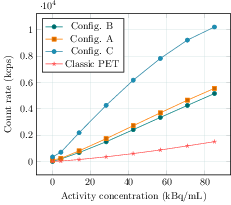
\includegraphics[width=0.5\linewidth]{allPrompts.png}}
    \subfloat[\label{fig:necr}]{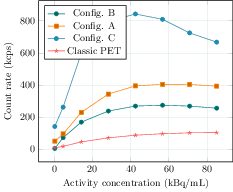
\includegraphics[width=0.5\linewidth]{allNECR.png}}
    \caption{From left to right: Prompt events detected by each configuration, NECR for each configuration.}
\end{figure}

\begin{figure}
    \centering
    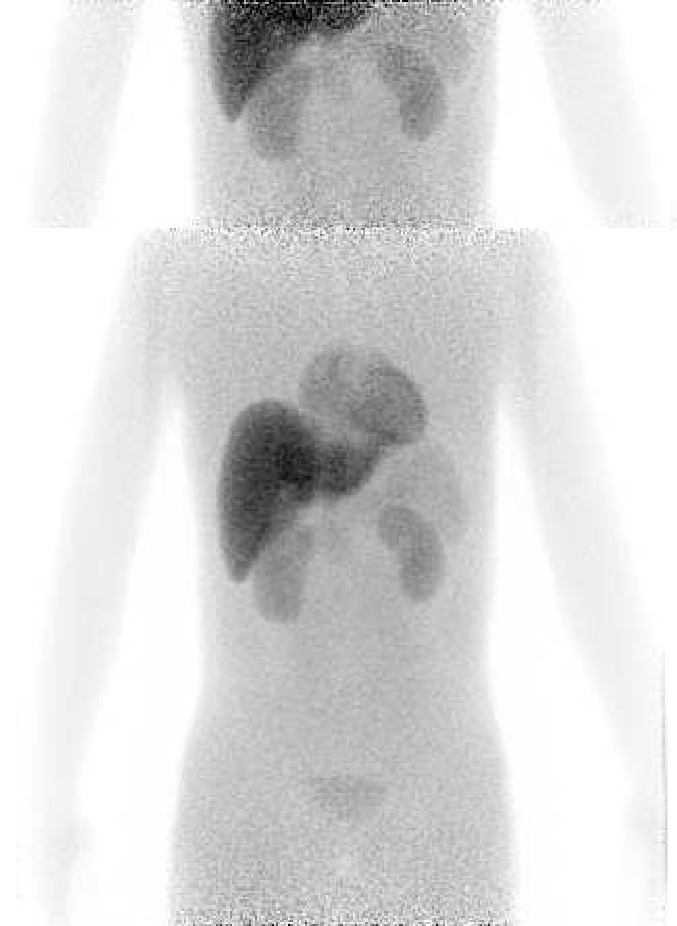
\includegraphics[width=0.85\linewidth]{recs.png}
    \caption{Images reconstructed with OSEM using $60$ iterations and $12$ subsets from top to bottom: from a classic PET scanner with a FOV of $240$mm and \texttt{Config.A}. Simulated from an XCAT phantom. Applied corrections: normalisation, attenuation, scatter. Randoms were excluded.}
    \label{fig:recs}
\end{figure}

\section{Conclusion}
An alternative cost efficient design for a TB-PET scanner using a chess-like pattern of detectors was evaluated, in terms of count losses. This was compared to a compact configuration having the same number of detectors and a configuration with the same axial length and double the detectors. It was found that although the impact on the counting ability of the scanner is not significant the NECR is reduced by $25\%$. This hints that the detected true events suffer greater losses than the random and scattered. 

Currently our ability to reconstruct images of long PET scanner maxes out at $700$mm. In the future we plan to further extend that using more efficient memory management. 

\AtNextBibliography{\small}
\printbibliography

\end{document}
